\documentclass{article}
\textheight 23.5cm \textwidth 15.8cm
%\leftskip -1cm
\topmargin -1.5cm \oddsidemargin 0.3cm \evensidemargin -0.3cm
%\documentclass[final]{siamltex}

\usepackage{ctex}
\usepackage{verbatim}
\usepackage{fancyhdr}
\usepackage{graphicx}
\usepackage{amsmath}
\usepackage{amssymb}
\usepackage{float}
\usepackage{multirow}
\usepackage{colortbl}
\usepackage{amsthm}
\usepackage{bm}
\usepackage{tikz}

\textheight 23.5cm \textwidth 15.8cm
\topmargin -1.5cm \oddsidemargin 0.3cm \evensidemargin -0.3cm
\title{HW8 实验报告}
\author{PB20010429 侯相龙}

\begin{document}
\maketitle
\section{实验内容}
实现 Bezier 曲线绘制


\section{实验原理}
基于Bernstein basis 构造Bezier 插值曲线,且其具有不同于一般多项式插值的convex hull性质。

具体来说,假设待插值点为$\bm{p_1, p_2, \cdots, p_n}$, 则Bezier 曲线有如下形式:
\begin{equation}\label{eq1}
    \bm{f}(t)=\sum_{i=1}^n B_i^n\bm{p}_i,t\in[0,1]
\end{equation}

其中,$B_i^{n}(t) = \binom{n}{i}t^i(1-t)^{n-i}$.

\section{算法介绍与步骤}
\begin{description}
    \item[1)]利用代数方法构造Bernstein basis.
    \item[2)]将插值点$\bm{p_i}$和采样点$t$代入公式(\ref{eq1}).
    \item[3)]绘制Bezier曲线,并研究其性质.

\end{description}


\section{测试数据与实验结果}
交互界面选取不同的插值点,实验结果如下:

\begin{figure}
    \caption{基于五点插值的Bezier曲线}
    \begin{center}
       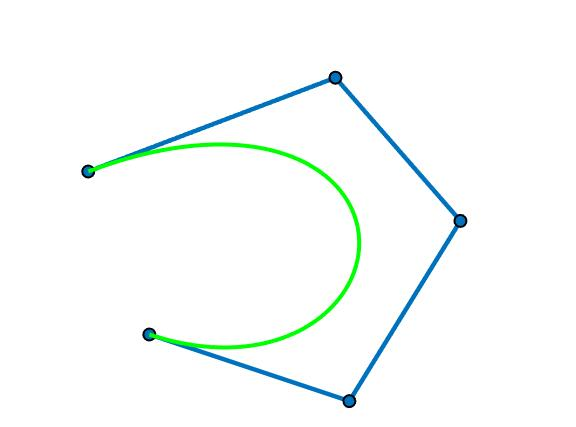
\includegraphics[width=0.5\linewidth]{1} 
    \end{center}
\end{figure}

\begin{figure}
    \caption{Bezier曲线的凸包性质}
    \begin{center}
       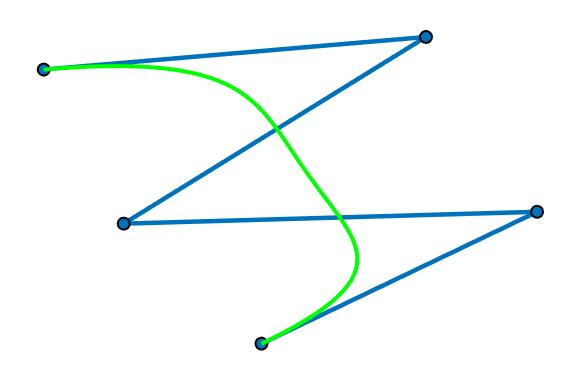
\includegraphics[width=0.5\linewidth]{2} 
    \end{center}
\end{figure}




\end{document}
